\newpage
\section{柔軟外皮を備えたワイヤ駆動式魚ロボットの開発}
\subsection{本研究の目的}
前章で述べたように,先行研究\cite{kyu}では屈曲可能な胴体を持ち,柔軟外皮を装着して完全防水を可能にした魚ロボットの開発に成功した.しかし,リンクと外皮に隙間ができてしまい,
リンクの動きを外皮にうまく伝えることができなかった.そこで本研究では魚らしいしなやかな動きを可能にするワイヤ駆動式の魚ロボットをベースにリンクに外皮を追従させ,尾びれのみならず
胴体部まで振って泳ぐことが可能なロボットの開発を目指す.さらに外皮の有無による遊泳性能の向上の変化について実機実験によって検証する.

\subsection{ワイヤ駆動式魚型ロボットの動作原理}
昨年度卒業研究で提案され,本研究でも採用したワイヤ駆動の動作原理を記す.ロボット前方にはプーリを取り付けたサーボモータを配置し,胴体部には弾性体とそれに固定した骨格リンクを配置する.
ワイヤはプーリーから骨格リンクに設けられた穴を通って尾びれ付け根まで伸びており,プーリーを回してワイヤを巻き取ることによって弾性体が曲がり,胴体部を屈曲させることができる.それを左
右に繰り返すことで遊泳を可能にする(図\ref{fig:waiyakudou})

\begin{figure}[b]
   \centering
   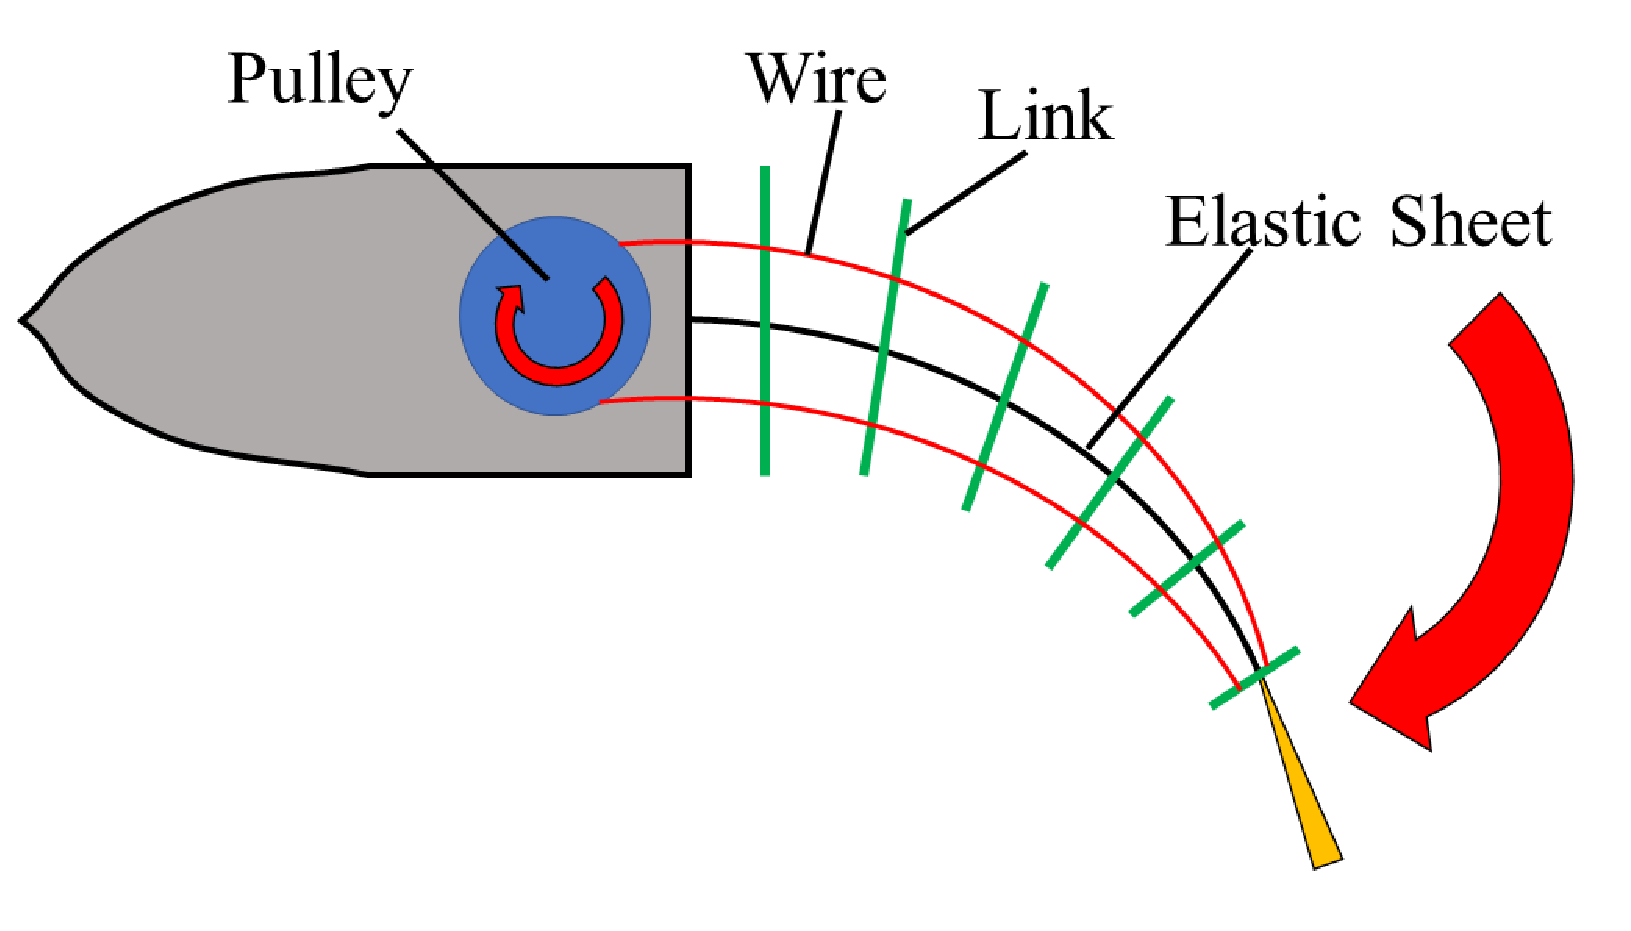
\includegraphics[width=0.6\linewidth]{chapters/picture/waiyakudou.eps}
   \caption{ワイヤ駆動のイメージ}
   \label{fig:waiyakudou}
\end{figure}

\subsection{試作機}
\subsubsection{試作機の作製}
まず,昨年度卒業研究を参考にして試作機を作製した.図\ref{fig:sisaku}に外観を,図\ref{fig:kouzou_sisaku}に構造を示す.全長は530 mm,重量は478 gである.試作機は頭部と胴体部の二つ
の部分で構成している.

頭部には制御回路とバッテリーを搭載しており,えらにあたる部分には防水仕様(IP67)の サーボモータ(Flash Hobby, M45CHW)を配置している.使用マイコンはM5Stamp Pico(M5Stack Technology 社),
使用バッテリーはマイコン用の3.7 V,サーボモータ用の7.4 Vの二つのLi-ionバッテリーを使用している.そのため,頭部は防水が必要となり,頭部の断面にOリングをはめ込むことによって防水を行っている.
頭部はネジ穴が空いたものと,ナット用の穴が空いたものに分かれており,これらはM1.7ネジで固定される.
胴体部は骨格リンク(PLA樹脂)と弾性体(ポリプロピレン板,厚さ0.75 mm),尾びれ(TPU樹脂,厚さ2 mm)で構成されており,骨格リンクは図のように楕円形にして作製し,ワイヤ(ポリエステル製,0.40 mm)
を通す穴を空けている.

\begin{figure}[t]
    \centering
    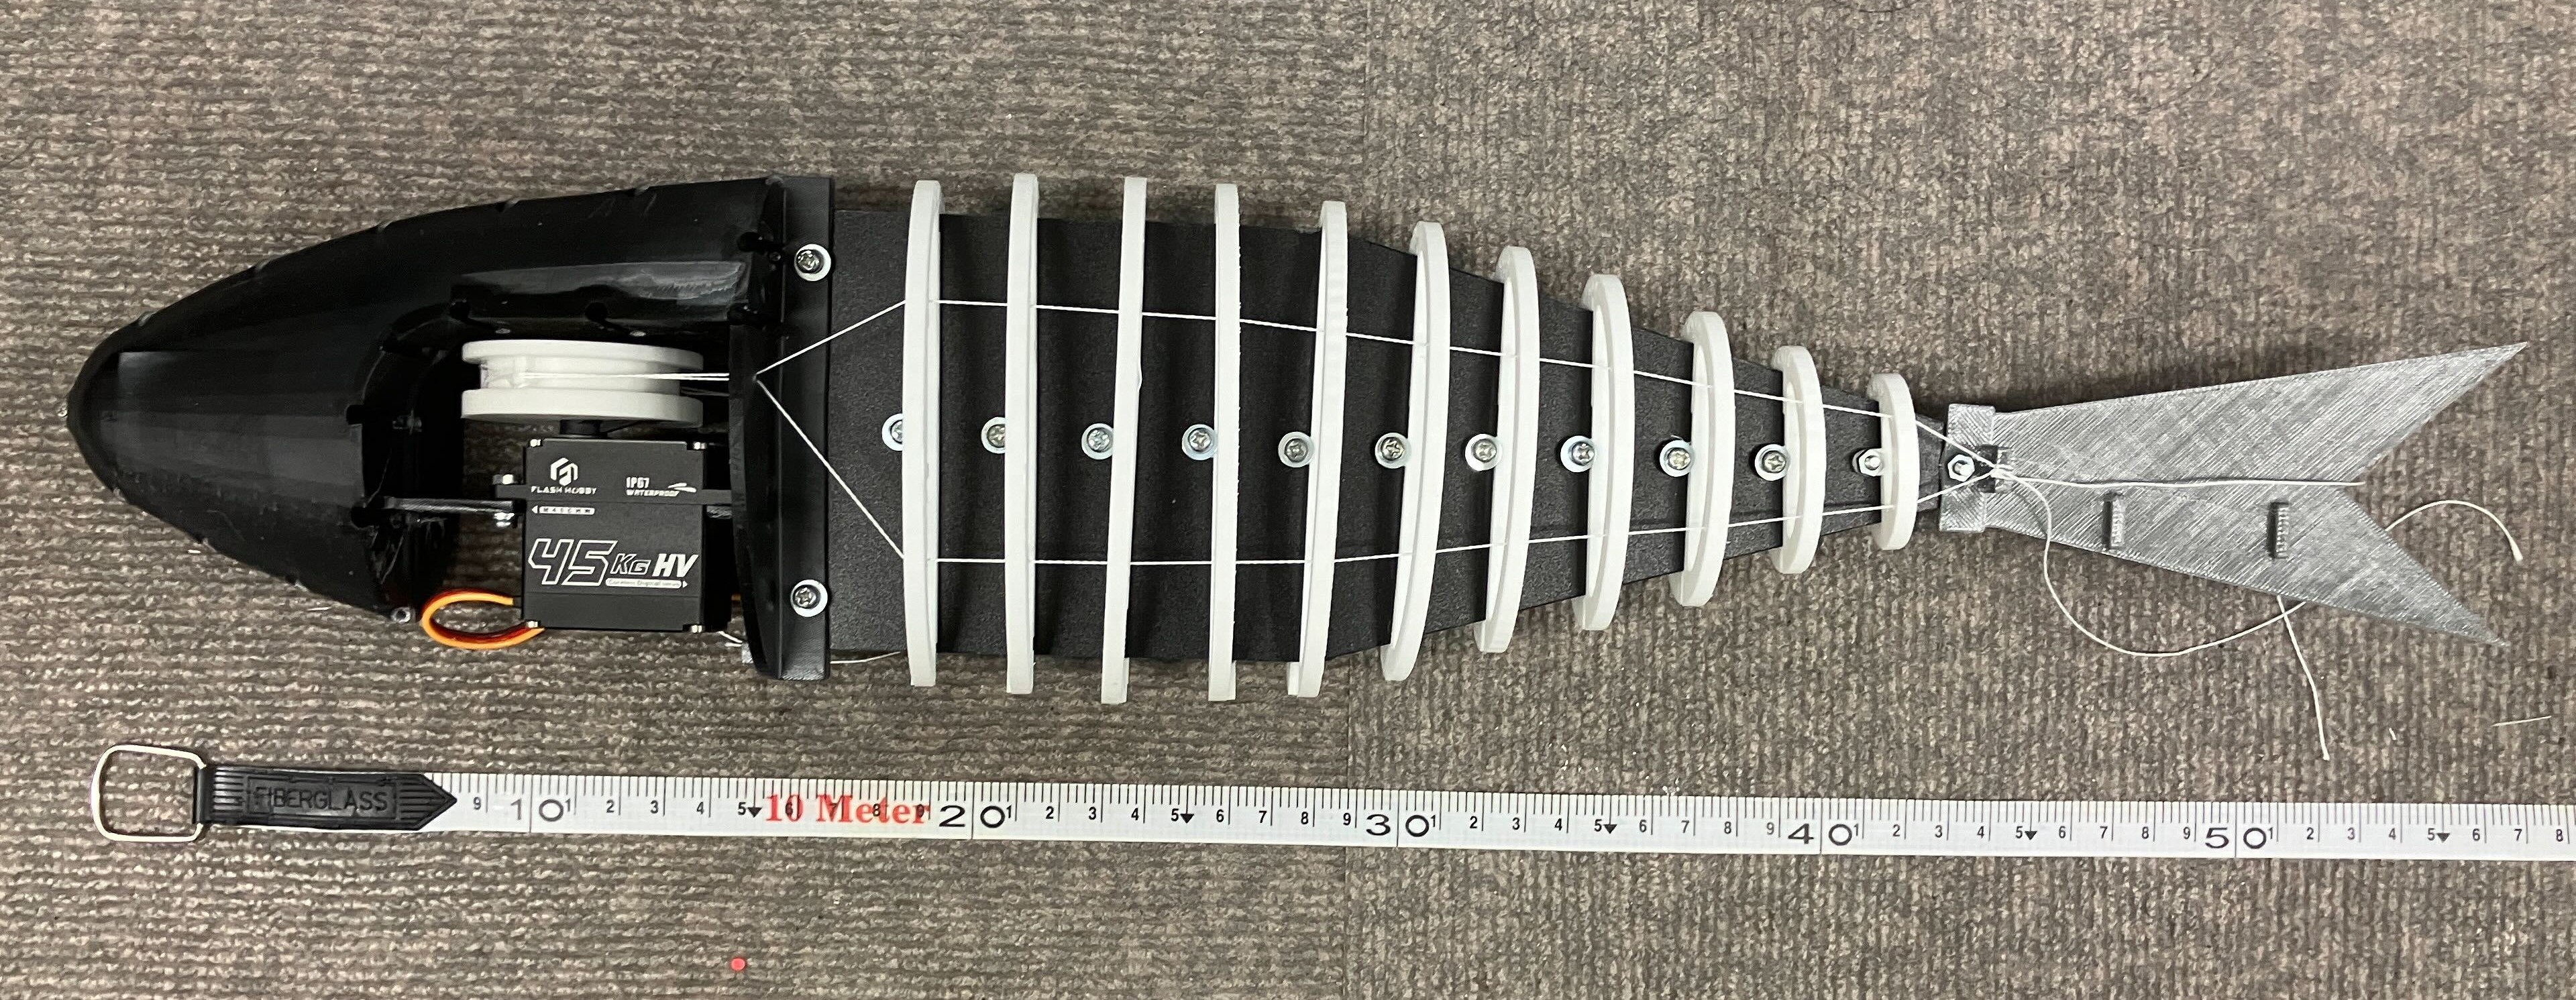
\includegraphics[width=0.80\linewidth]{chapters/picture/sisaku.jpg}
    \caption{試作機の外観}
    \label{fig:sisaku}
\end{figure}
\begin{figure}[t]
    \centering
    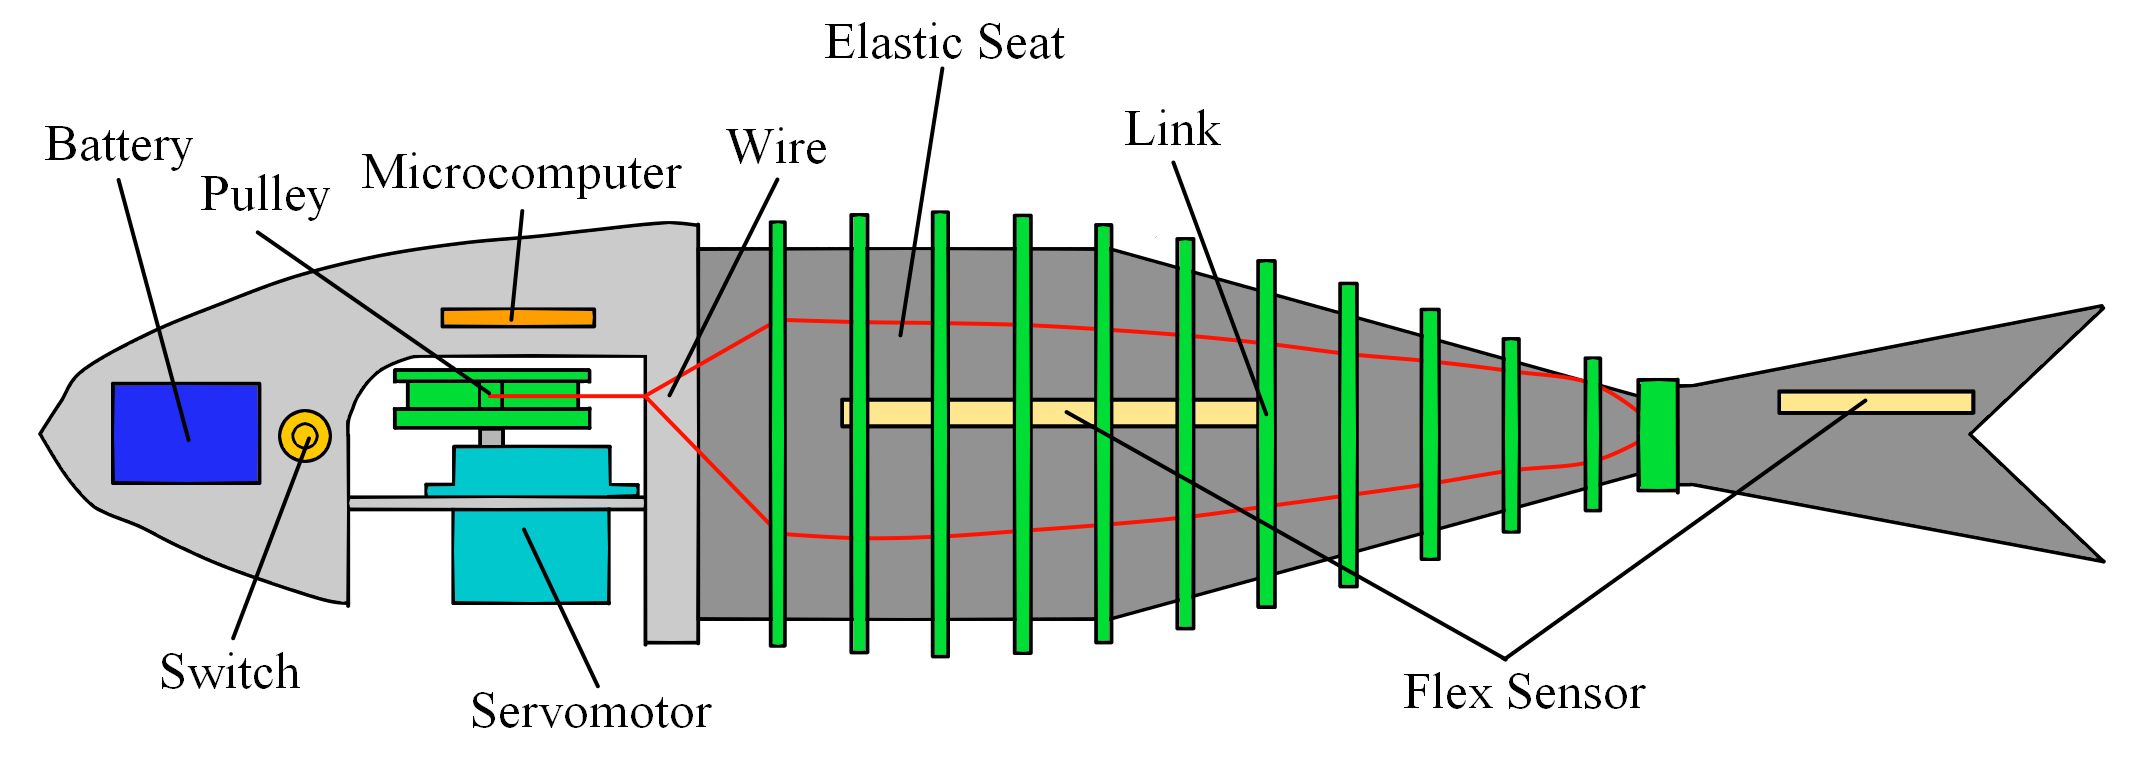
\includegraphics[width=0.80\linewidth]{chapters/picture/tentativeschematic.png}
    \caption{試作機の構造}
    \label{fig:kouzou_sisaku}
\end{figure}
\begin{figure}[t]
    \centering
     \begin{minipage}[b]{0.50\linewidth}
        \centering
        \setPicture{ring.jpg}
        \caption{頭部断面のようす}
        \label{fig:danmen}
     \end{minipage}
     \hspace{0.05\linewidth}
     \begin{minipage}[b]{0.25\linewidth}
        \centering
        \setPicture{jikkilink.png}
        \caption{骨格リンク}
        \label{fig:link_sen}
     \end{minipage}
\end{figure}

\subsubsection{防水テスト・遊泳テスト}
機体完成後,防水テストと遊泳テストを行った.まず防水テストは水没すると赤くなるシールを頭部内部に貼り,水深120 mmの水槽で2 分間沈める防水テストを7回行った.それぞれねじの締め具合や
頭部の歪みを直しながらテストをしたが,完全な防水はできず,7回目で頭部下方のみの浸水にとどまったのでこれで防水できていると判断した(図\ref{fig:bousuitest_sisaku}).
次に遊泳テストを行った.遊泳テストの様子を図\ref{fig:test_sisaku}に示す.

\begin{figure}[t]
    \centering
    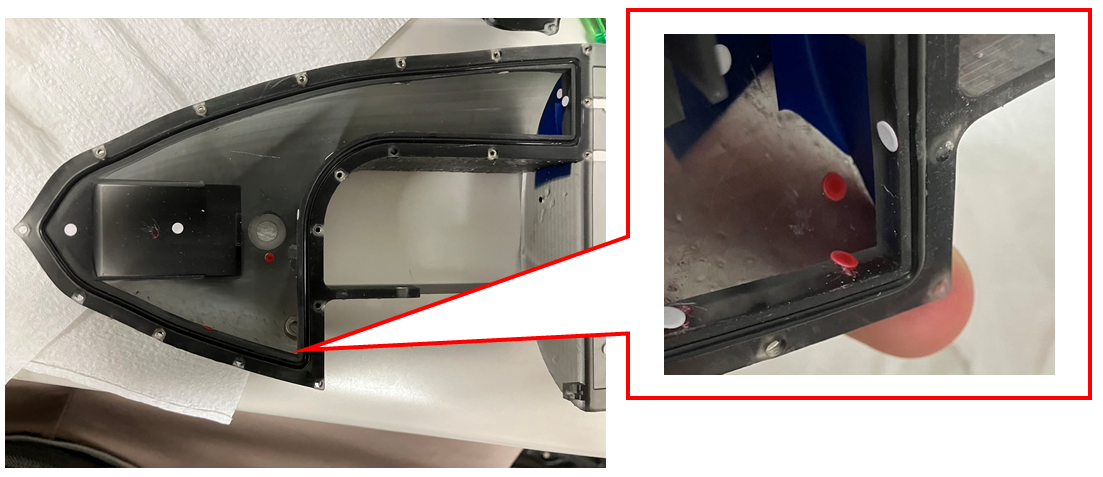
\includegraphics[width=0.80\linewidth]{chapters/picture/bousuitest.png}
    \caption{頭部下方浸水のようす}
    \label{fig:bousuitest_sisaku}
\end{figure}
\begin{figure}[t]
    \centering
    \setPicture{sisakuoyogu2.png}
    \caption{遊泳テストの様子}
    \label{fig:test_sisaku}
\end{figure}

\subsubsection{試作機から得られた知見}
試作機の作製・動作確認を通して得られた知見として,まず,頭部をネジとOリングを用いて防水する方法は完全な防水に至らないと考えられる.また,頭部を固定するネジが多いと,バッテリー交換が
しにくく,メンテナンス性が悪くなるということも分かった.以上のことから防水方法を変更し,メンテナンス性を向上させた頭部に改良することが必要だとわかった.

\newpage

\subsection{ワイヤ駆動式柔軟外皮装着型魚ロボットの開発}
ここからは本研究で開発した機体について述べる.
図\ref{fig:fishrobo_with}に開発した機体の外観を,図\ref{fig:kouzou}に構造を示す.開発した魚ロボットは体長470 mm,重量は重り(25 g)を含めて710 gである.ロボットの外形は
昨年度卒業研究においてアジのスキャンデータ(図\ref{fig:data_scan})から作製したモデルデータ(図\ref{fig:data_model})をもとに作製し,サイズは2倍とした.本機体は頭部・胴体
部・外皮の3つからなり,頭部と胴体部をそれぞれ別の柔軟外皮で包む構造になっている.また,頭部は防水区画とし,胴体部は水中姿勢を水平にするために浸水させた.

\begin{figure}[htbp]
    \centering  
    \begin{subfigure}[b]{0.9\linewidth}
        \centering
        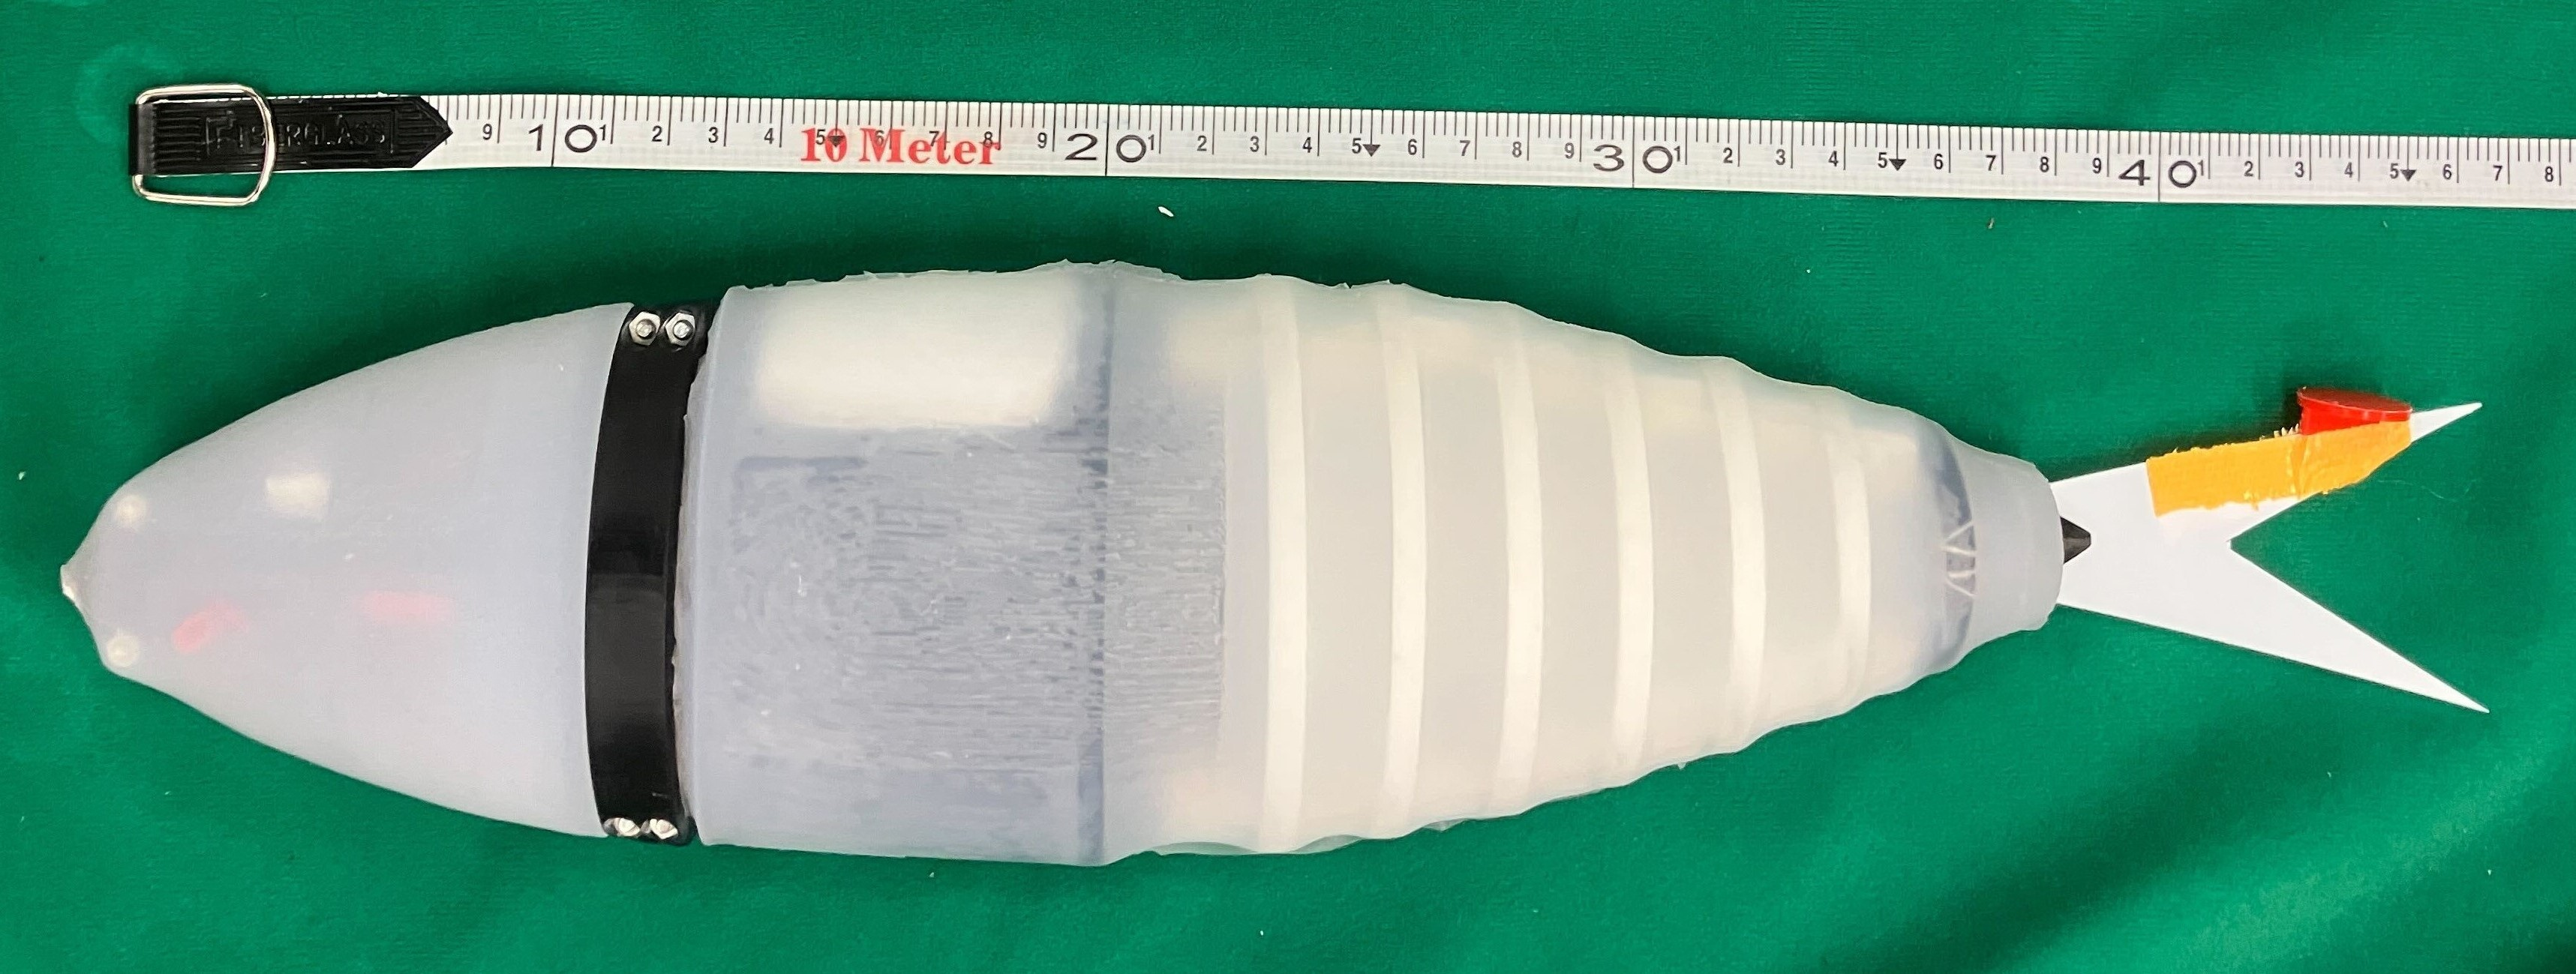
\includegraphics[width=0.9\linewidth]{chapters/picture/withskin.jpg}
        \subcaption{外皮あり}
        \label{fig:fishrobo_with}
    \end{subfigure}
    % \begin{subfigure}[b]{0.9\linewidth}
    %     \centering
    %     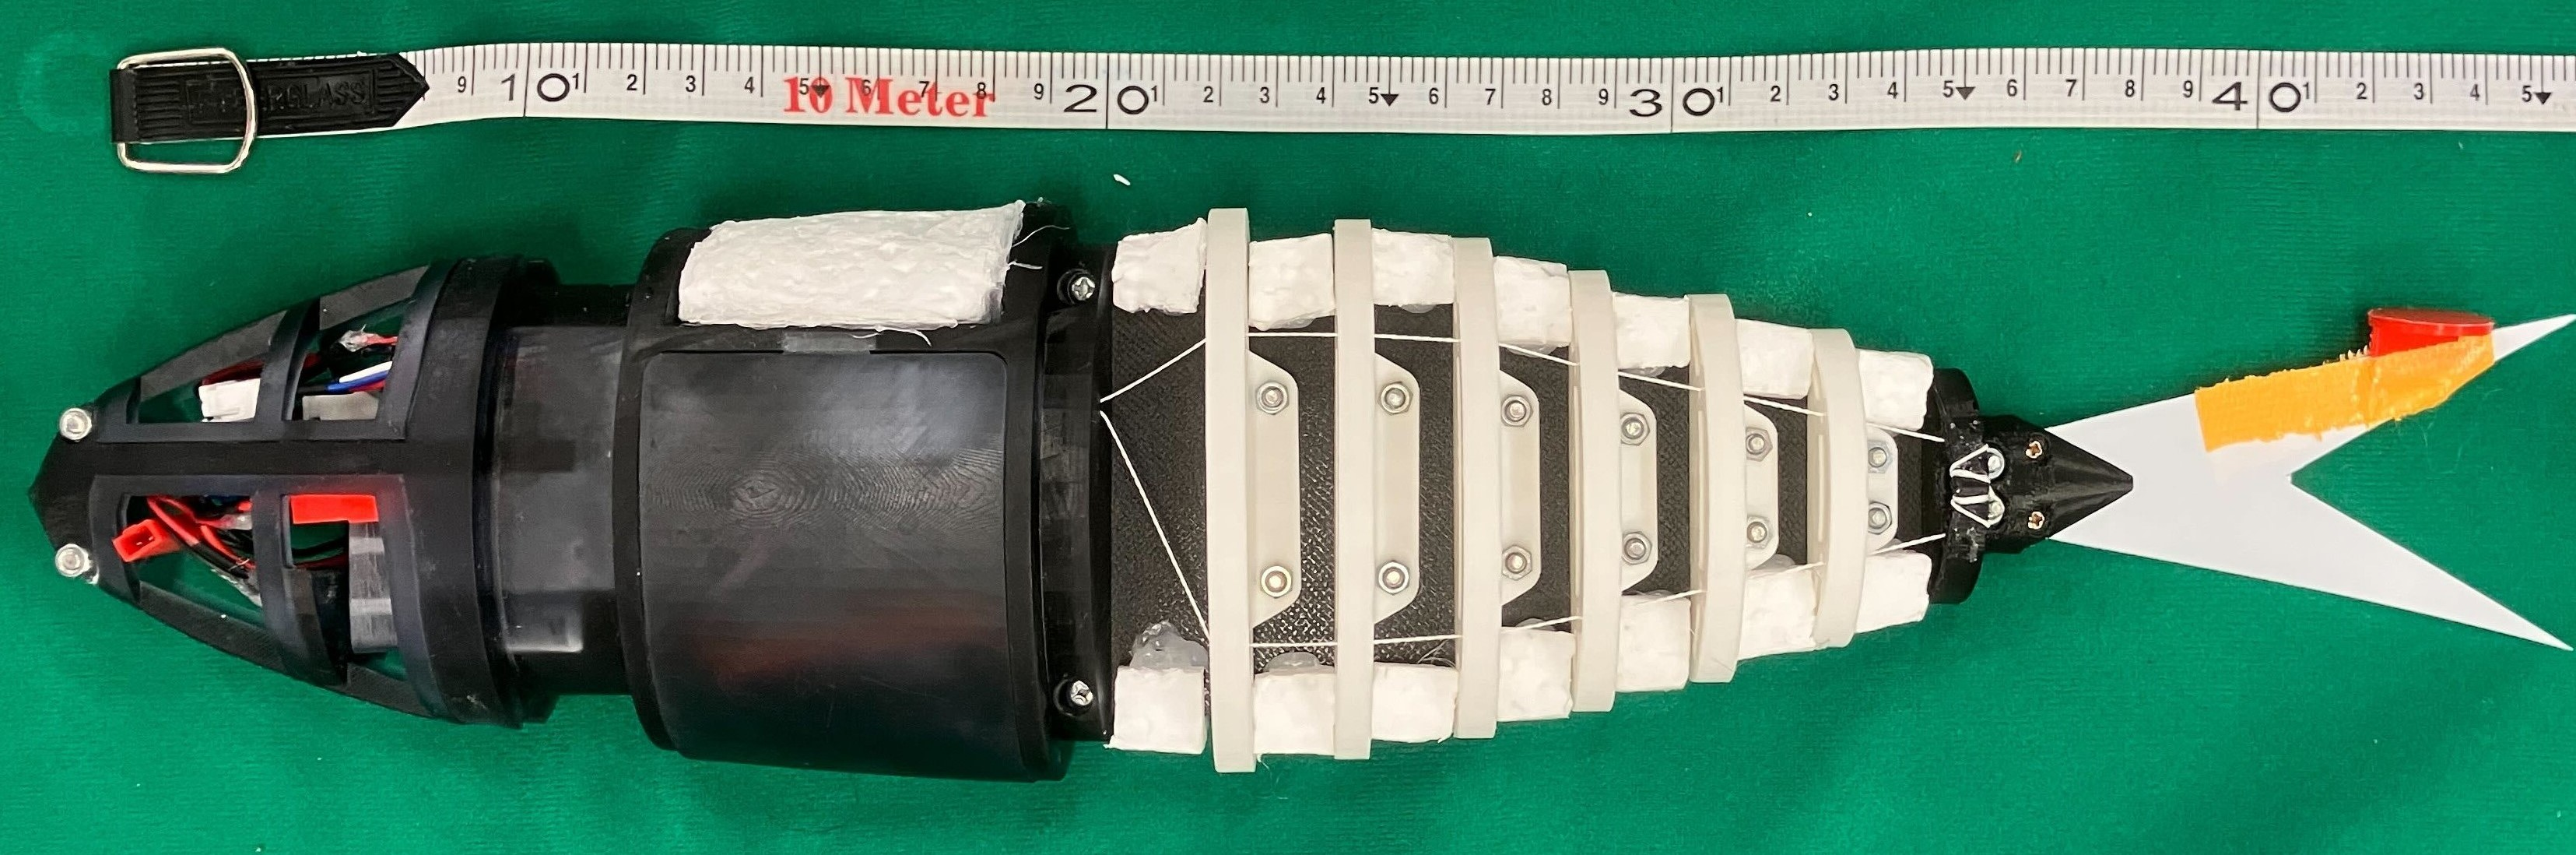
\includegraphics[width=0.9\linewidth]{chapters/picture/skinless.jpg}
    %     \subcaption{外皮なし}
    %     \label{fig:fishrobo_less}
    % \end{subfigure}
    \begin{subfigure}[b]{0.9\linewidth}
        \centering
        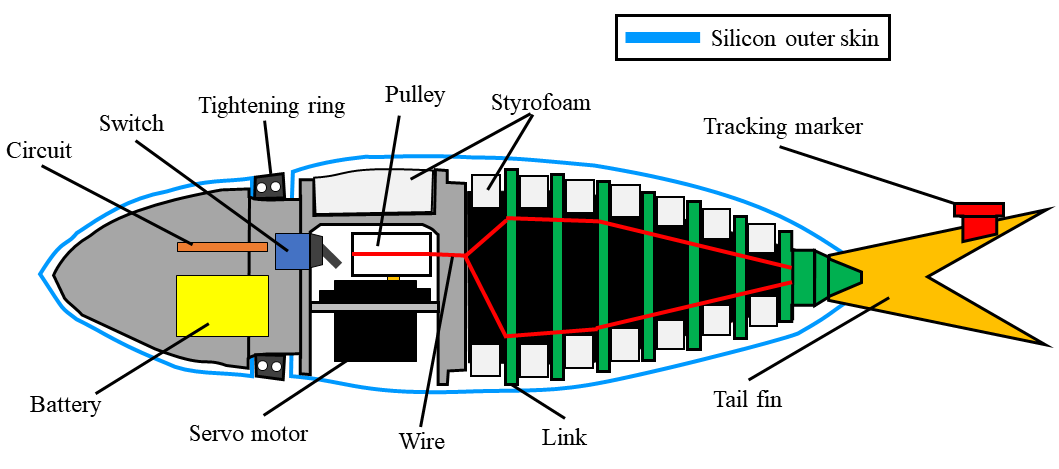
\includegraphics[width=0.9\linewidth]{chapters/picture/fish.png}
        \caption{開発したロボットの構造}
        \label{fig:kouzou}
    \end{subfigure}
    \caption{開発したロボット}
    \label{fig:gaikan}
\end{figure}
\begin{figure}[b]
    \centering
    \begin{minipage}[b]{0.4\linewidth}
        \centering
        \setPicture{skyan.png}
        \caption{アジのスキャンデータ}
        \label{fig:data_scan}
    \end{minipage}
    \hspace{0.05\linewidth}
    \begin{minipage}[b]{0.4\linewidth}
        \centering
        \setPicture{fishkinji.png}
        \caption{アジのモデルデータ}
        \label{fig:data_model}
    \end{minipage}
\end{figure}

\subsubsection{頭部}
頭部は光造形方式の3Dプリンタで作製しており,胴体前部と一体となっている.内部にはバッテリーと制御回路を搭載しており,使用するバッテリー,マイコン共に試作機と同じものを用いた.バッテリーと
マイコンを搭載する都合上頭部を防水する必要があり,試作機から得た知見をもとに今回はOリングによる防水ではなく,シリコン製の外皮を用いて防水を行った.
防水方法としてはシリコン製の外皮を頭部にかぶせ,根元を防水リングによって締め付けることで防水を行った(図\ref{fig:bousui}).防水リングのサイズは\cite{juuiti}を参考に締め付ける部分が
短径,長径ともに10%つぶせるように設計した.また,試作機と同様に防水実験を1回行ったが,内部に貼ったシールはどれも赤く染まらず,完全な防水ができた(図\ref{fig:bousui_test}).

\begin{figure}[htpb]
    \centering
    \begin{tabular}{cc}
        \begin{minipage}[b]{0.43\linewidth}
            \centering
            \setPicture{bousui.pdf}
            \subcaption{防水構造}
            \label{fig:bousui_kouzou} 
        \end{minipage}
        \begin{minipage}[b]{0.43\linewidth}
            \centering
            \setPicture{jissai.jpg}
            \subcaption{実際の様子}
            \label{fig:bousui_jissai} 
        \end{minipage}
    \end{tabular}
    \caption{頭部防水について}
    \label{fig:bousui}
\end{figure}
\begin{figure}[htbp]
    \centering
    \begin{tabular}{ccc}
        \begin{minipage}[b]{0.31\linewidth}
            \centering
            \setPicture{bousui_soku.jpg}
            \subcaption{頭部側面}
            \label{fig:toubu_soku}
        \end{minipage}
        \begin{minipage}[b]{0.31\linewidth}
            \centering
            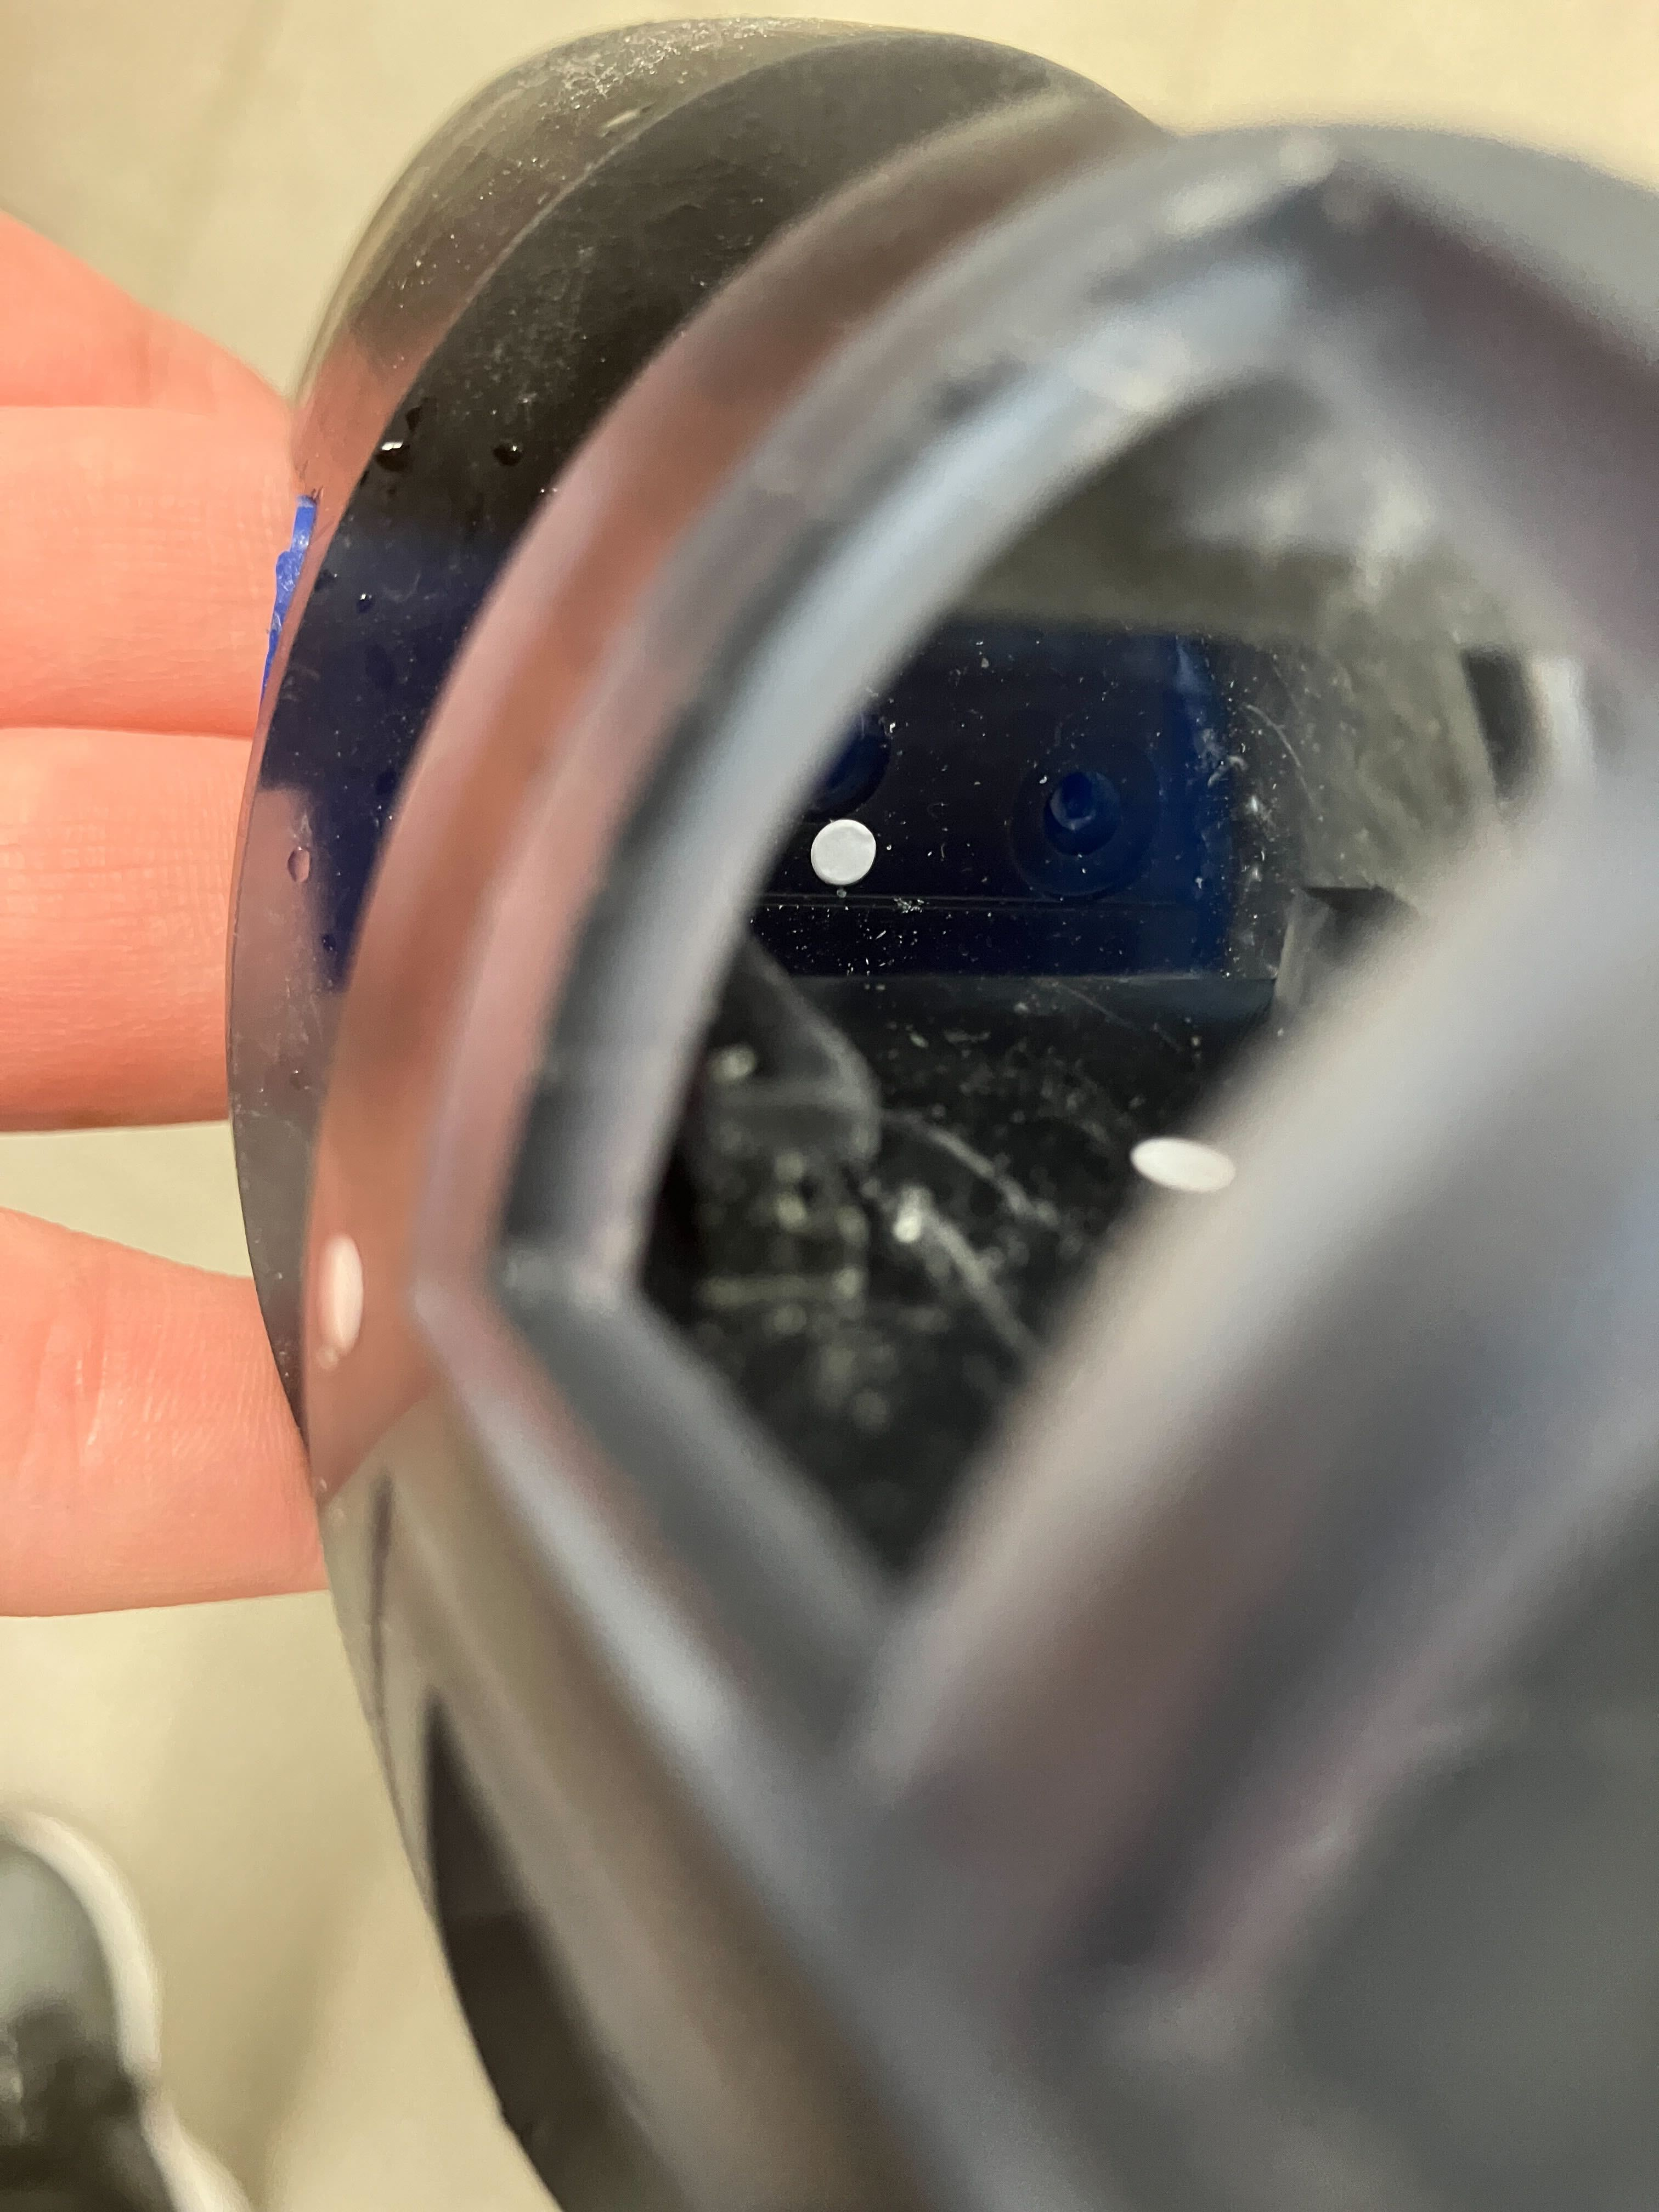
\includegraphics[width=0.8\linewidth]{chapters/picture/bousui_naka.jpg}
            \subcaption{頭部内側}
            \label{fig:toubu_uti}
        \end{minipage}
        \begin{minipage}[b]{0.31\linewidth}
            \centering
            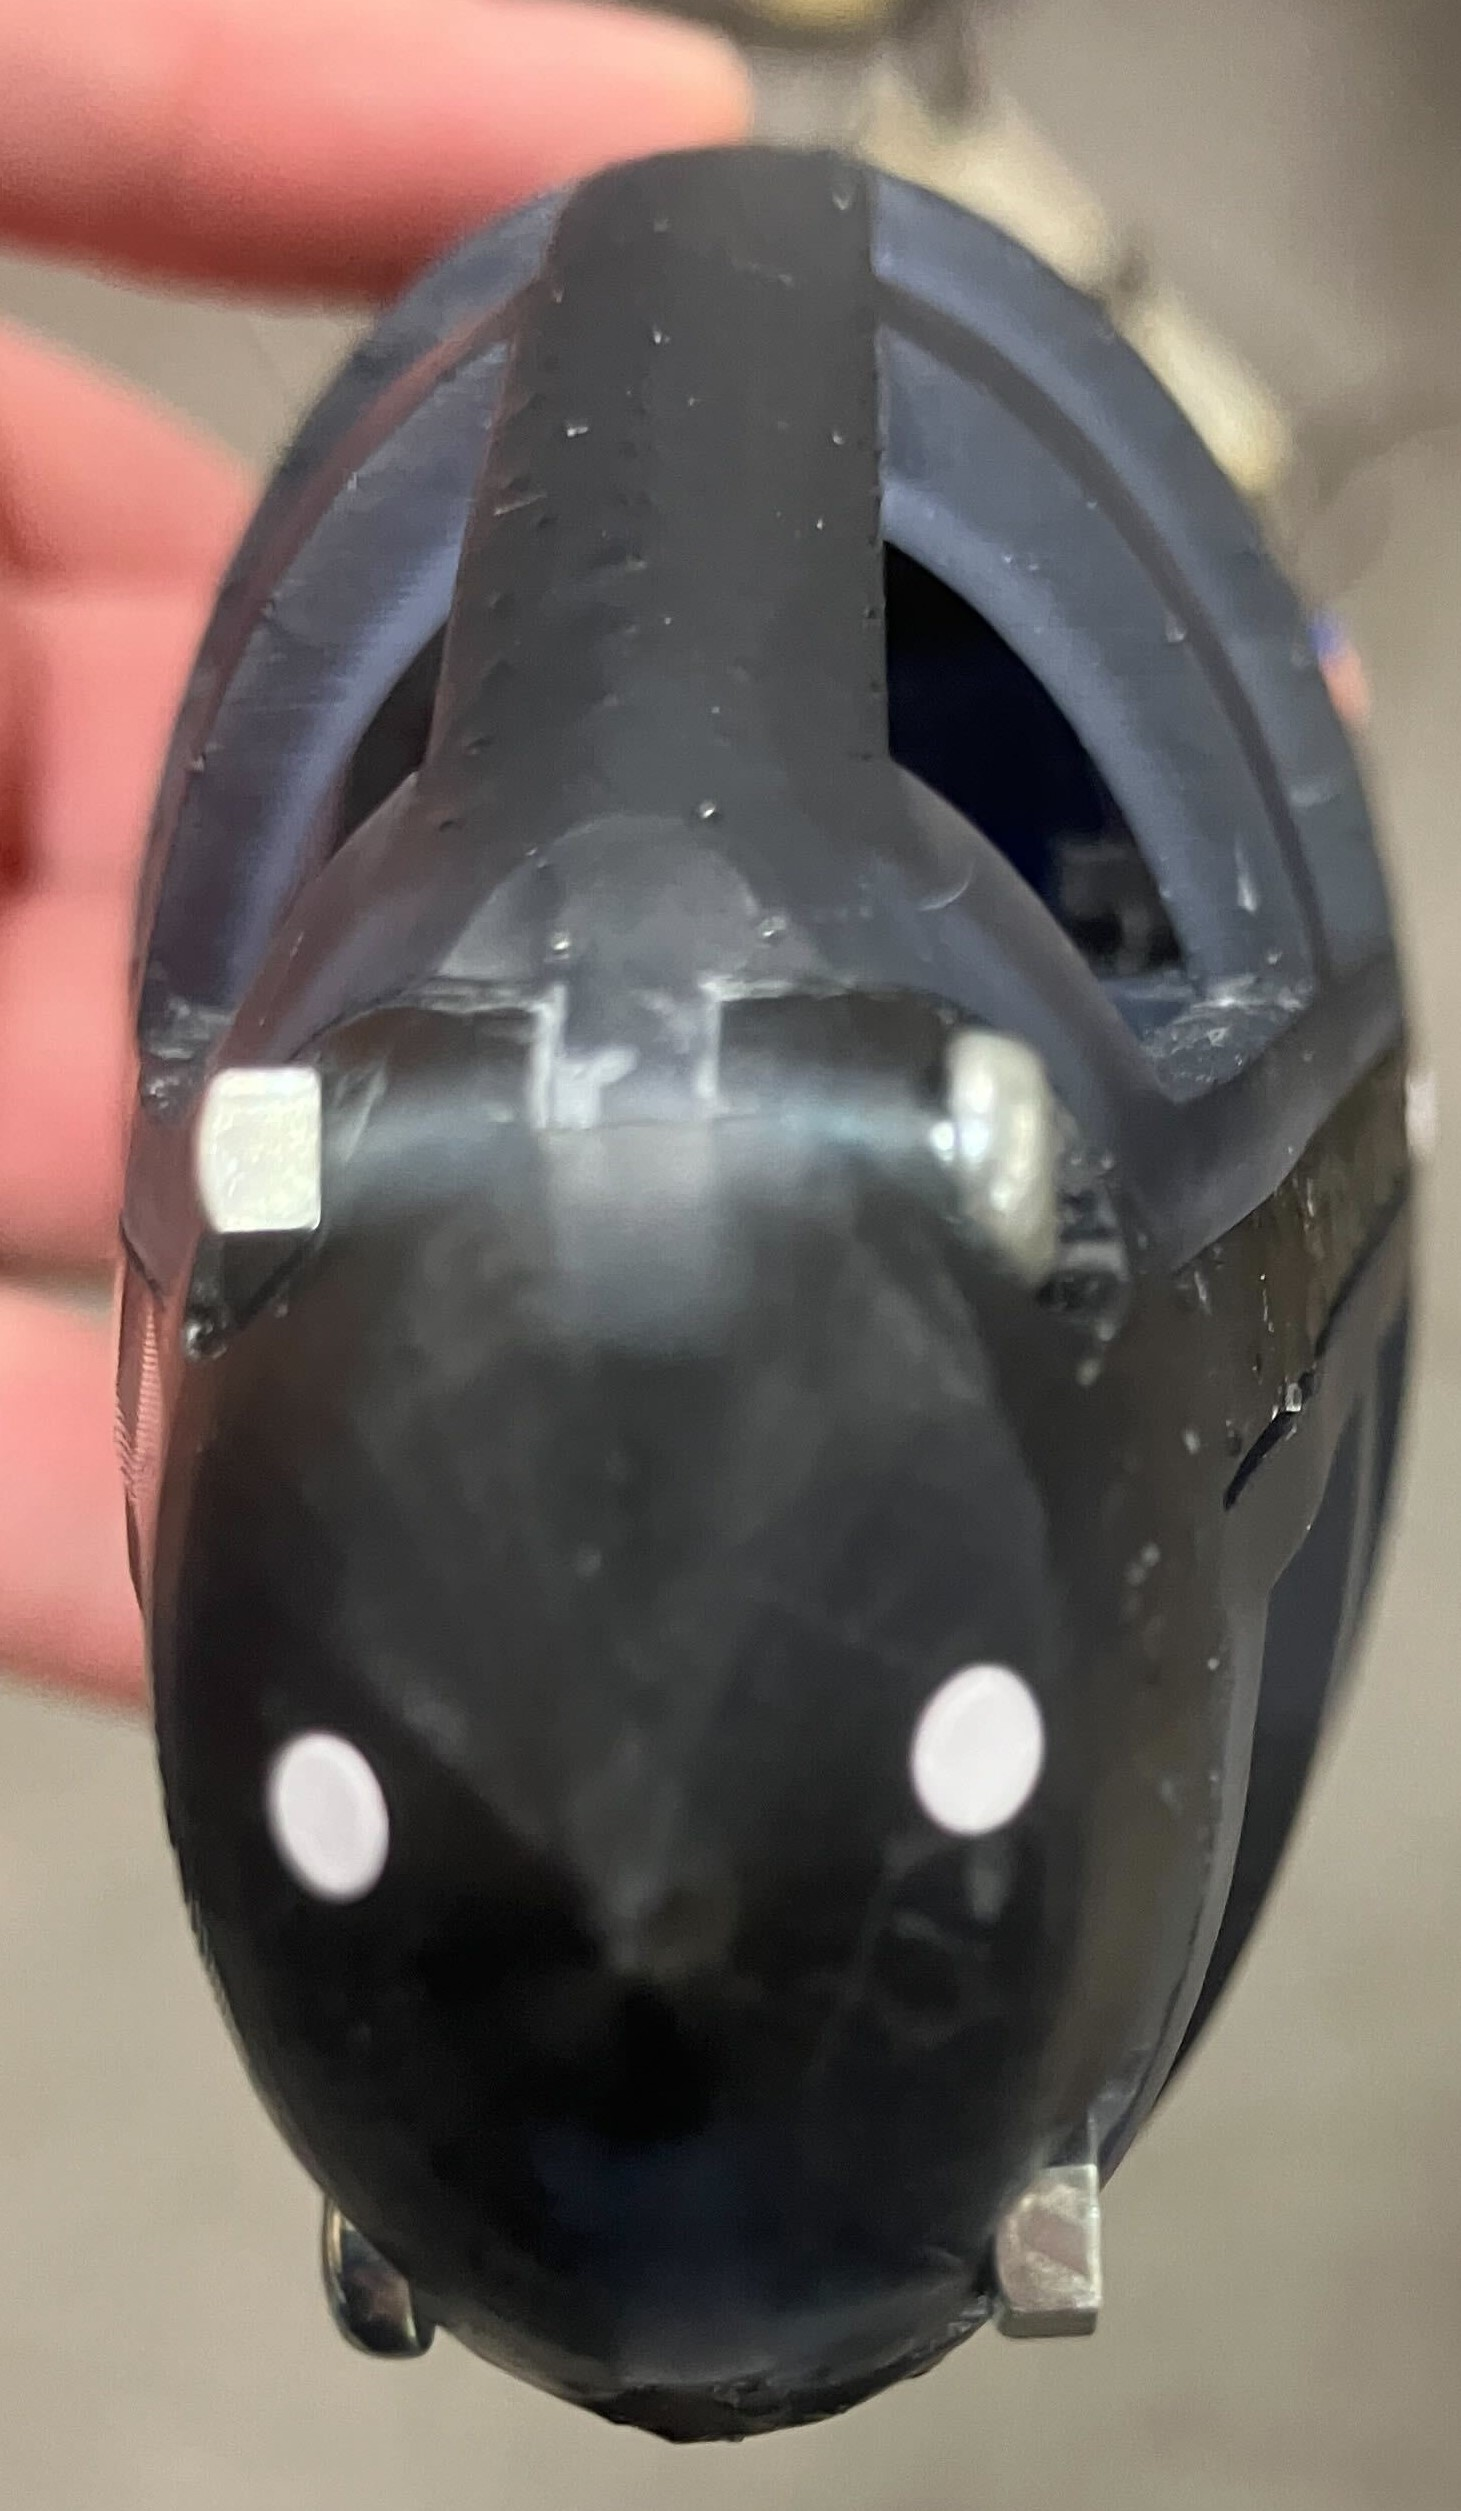
\includegraphics[width=0.7\linewidth]{chapters/picture/bousui_sentou.jpg}
            \subcaption{頭部先端}
            \label{fig:toubu_sentan}
        \end{minipage}
    \end{tabular}
    \caption{防水実験後のシールの様子}
    \label{fig:bousui_test}
\end{figure}

\newpage
また,頭部は上部と下部のカバーが開くようになっており,メンテナンス性向上のためにねじ止めではなくワンタッチでカバーを開閉できるようにしている
(図\ref{fig:head_open},\ref{fig:rock}).
それに加えて制御回路とバッテリーを取り出しやすくするためにねじで固定するのではなく,図\ref{fig:toubu_kiban},図\ref{fig:toubu_battery}のように溝にはめストッパーをつける
ことで頭部に配置している.

\begin{figure}[t]
    \centering
    \begin{minipage}[b]{0.3\linewidth}
        \centering
        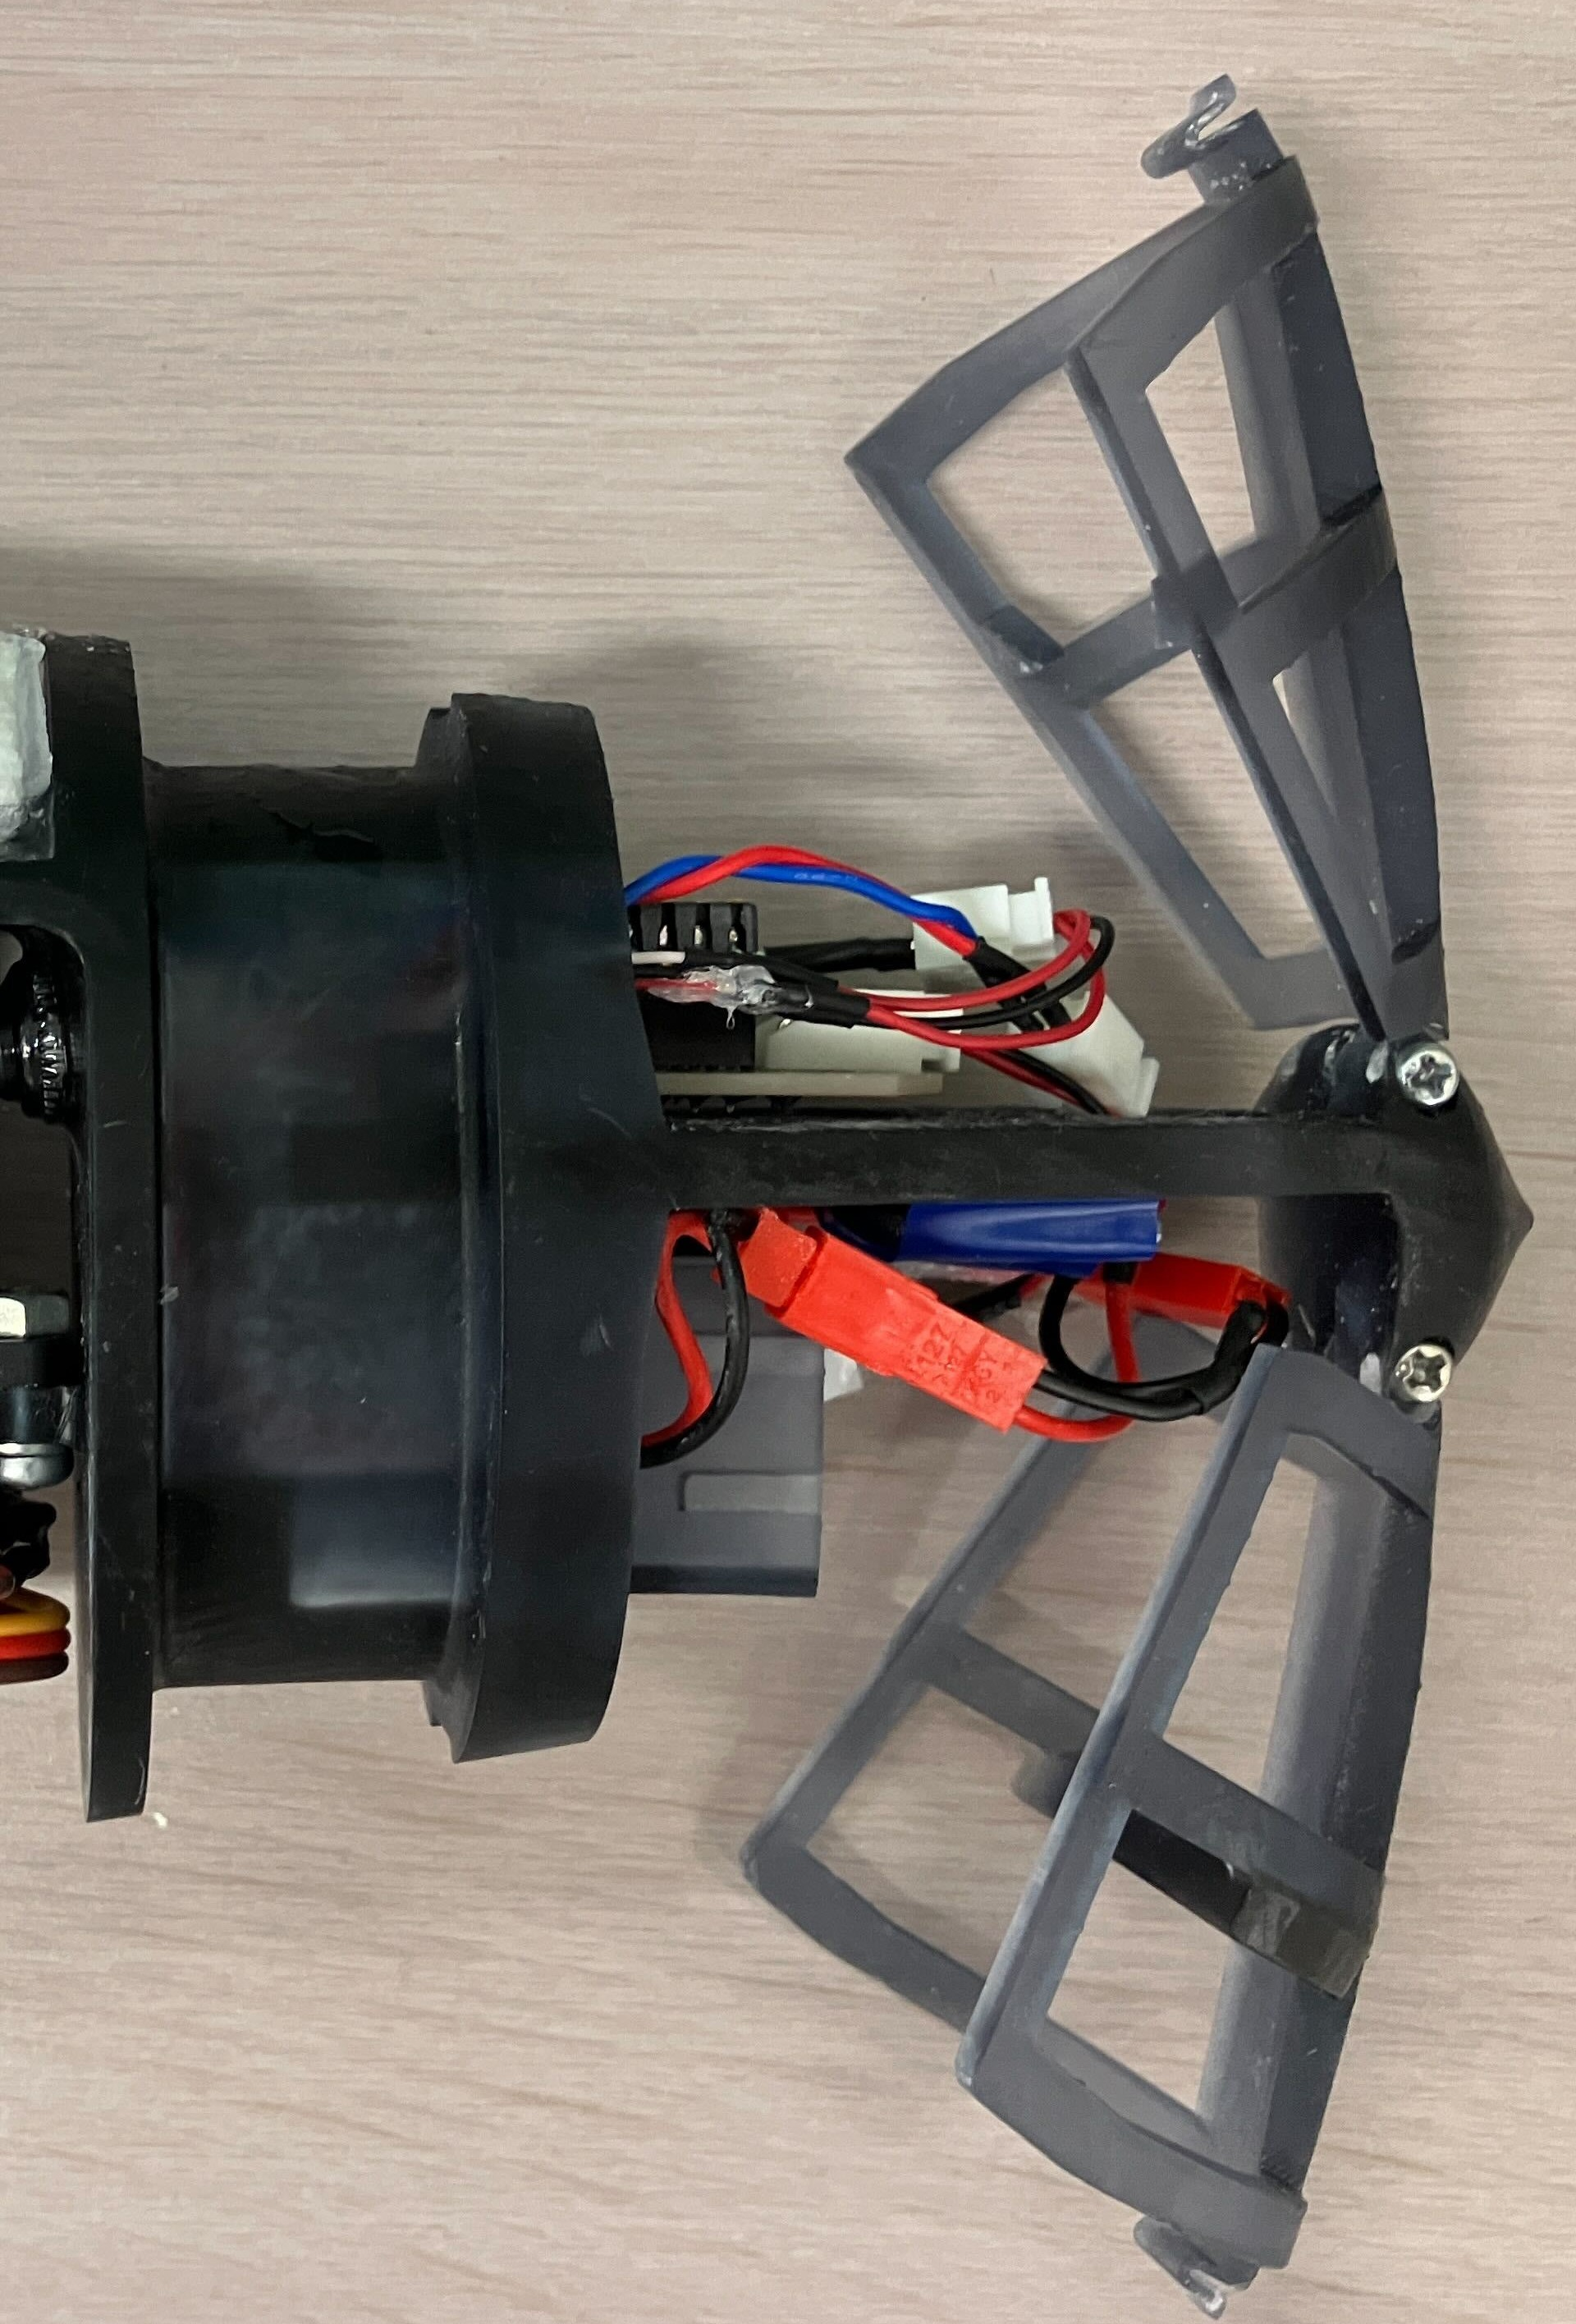
\includegraphics[width=0.6\linewidth]{chapters/picture/open_head.jpg}
        \caption{頭部開放時の様子}
        \label{fig:head_open}
    \end{minipage}
    \begin{minipage}[b]{0.5\linewidth}
        \centering
        \setPicture{rock.png}
        \caption{ワンタッチロックの仕組み}
        \label{fig:rock}
    \end{minipage}
\end{figure}
\begin{figure}[t]
    \centering
    \begin{minipage}[b]{0.4\linewidth}
        \centering
        \setPicture{toubu_kiban.png}
        \caption{基板固定方法}
        \label{fig:toubu_kiban}
    \end{minipage}
    \hspace{0.1\linewidth}
    \begin{minipage}[b]{0.4\linewidth}
        \centering
        \setPicture{toubu_battery.png}
        \caption{バッテリー固定方法}
        \label{fig:toubu_battery}
    \end{minipage}
\end{figure}

\subsubsection{胴体部}
胴体部は細かく分けて駆動部,弾性体部,尾びれ部で構成されている.
駆動部は頭部と一体化しており,試作機と同じサーボモータを配置し,プーリー(PLA樹脂)を取り付けている.また,サーボモータの信号線を制御回路側につなげるために防水キャプコン
(オーム電機,OA-WS04M-20/25)を配置し,さらに電源スイッチも配置している(図\ref{fig:kudou}).また,駆動部には図\ref{fig:cover}のようなカバーをかぶせ魚らしい形状になるようにしている.

弾性体部は弾性体(ポリプロピレン板,厚さ0.75 mm)と骨格リンク(PLA樹脂),ワイヤ(ポリエステル製,0.40 mm)で構成している.骨格リンクは厚みを6mmで作製し,14 mm間隔を空
けながら配置した.リンクには図のようにワイヤを通すために2 mmの穴を4 カ所開けており,さらに胴体内部を浸水させるために大きめの穴を6 個開けている(図\ref{fig:link2}).また,リンクと弾性体は
ネジを用いて二点止めし,外皮の動きがリンクの固定状態に影響を与えないようにした(図\ref{fig:real_link}).

尾びれ部は図\ref{fig:obire}のように尾びれ本体(ポリスチレン製薄板,厚さ0.3 mm)と骨格リンクの一部で構成している.尾びれに関しては先行研究より推進性能が高いと示された材料と厚みを使用して
おり,形状に関してはアジの3Dスキャンデータからサイズを決定した.骨格リンクは尾びれを固定するための固定部を設け,尾びれが折れないようにTPU樹脂で作製し,根元を三角形状にすることで折り目がつ
かないようにした.

\begin{figure}[t]
    \centering
    \begin{minipage}[b]{0.35\linewidth}
        \centering
        \setPicture{kudou.png}
        \caption{駆動部のようす}
        \label{fig:kudou}
    \end{minipage}
    \hspace{0.1\linewidth}
    \begin{minipage}[b]{0.35\linewidth}
        \centering
        \setPicture{cover.jpg}
        \caption{駆動部カバー}
        \label{fig:cover}
    \end{minipage}
\end{figure}
\begin{figure}[t]
    \centering
    \begin{minipage}[b]{0.35\linewidth}
        \centering
        \setPicture{link2.png}
        \caption{骨格リンクについて}
        \label{fig:link2}
    \end{minipage}
    \hspace{0.1\linewidth}
    \begin{minipage}[b]{0.35\linewidth}
        \centering
        \setPicture{link_danseita.jpg}
        \caption{実際の弾性体部}
        \label{fig:real_link}
    \end{minipage}
\end{figure}
\begin{figure}[t]
    \centering
    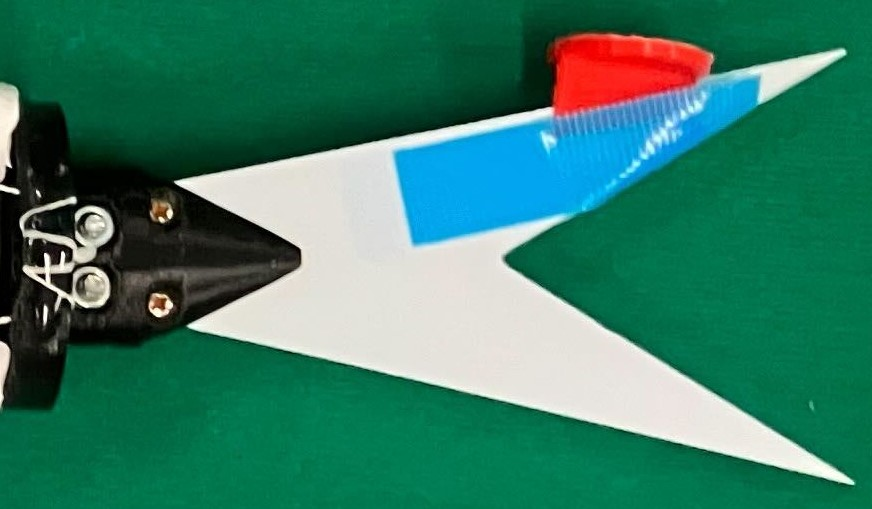
\includegraphics[width=0.6\linewidth]{chapters/picture/obire.jpg}
    \caption{尾びれ部}
    \label{fig:obire}
\end{figure}

\subsubsection{外皮}
柔軟外皮は頭部と胴体部用に二つ作製した.今回は外皮を作製するため鋳造のように型にシリコンを流し入れることによって外皮の作成を行った.図\ref{fig:katanaka}に作製・使用した型
と中子をそれぞれ示す.ここで中子とは鋳造において中空部を作るために使われているもので, 型の間にはめ込んで使用する.この制作方法において外皮の外寸サイズを決定するのは型に作る
くぼみ,内寸サイズを決定するのは中子となる.したがってここから型のくぼみのサイズを外皮の外寸,中子のサイズを外皮の内寸と呼ぶ.

まず頭部用の外皮について,外皮の内寸は外皮と頭部が密着するようにアジの3Dモデルの頭部のサイズをそのまま使用した.外寸については体高方向に2 mm,体幅方向に3 mmの厚みになるよう
にアジのモデルデータの頭部をx軸方向に1.15 倍,y軸方向に1.09 倍,z軸方向に1.07 倍したサイズを使用した.

次に胴体部の外皮ついて述べる.リンクの動きに外皮を追従させるために外皮内部に骨格リンクをはめ込めるような溝を作製し,しわができないように外皮の内寸をロボットの胴体サイズの90 %
のサイズで作製した.溝の間隔もロボット胴体サイズの90 %になるようにリンク間距離14 mmの90 %の長さにあたる12.6 mm間隔で作製した.溝の深さは骨格リンクに通すワイヤに干渉しないかつ溝か
ら外れないように5 mmで設計した.
図\ref{fig:gaihi}に作製した外皮を示す.

\begin{figure}[hb]
    \centering
    \begin{tabular}{cc}
        \begin{minipage}[b]{0.43\linewidth}
            \centering
            \setPicture{atata.jpg}
            \subcaption{頭部外皮用の型と中子}
            \label{fig:atata} 
        \end{minipage}
        \hspace{0.05\linewidth}
        \begin{minipage}[b]{0.43\linewidth}
            \centering
            \setPicture{katata.jpg}
            \subcaption{胴体外皮用の型と中子}
            \label{fig:katata} 
        \end{minipage}
    \end{tabular}
    \caption{作製した型と中子}
    \label{fig:katanaka}
\end{figure}
\begin{figure}[b]
    \centering
    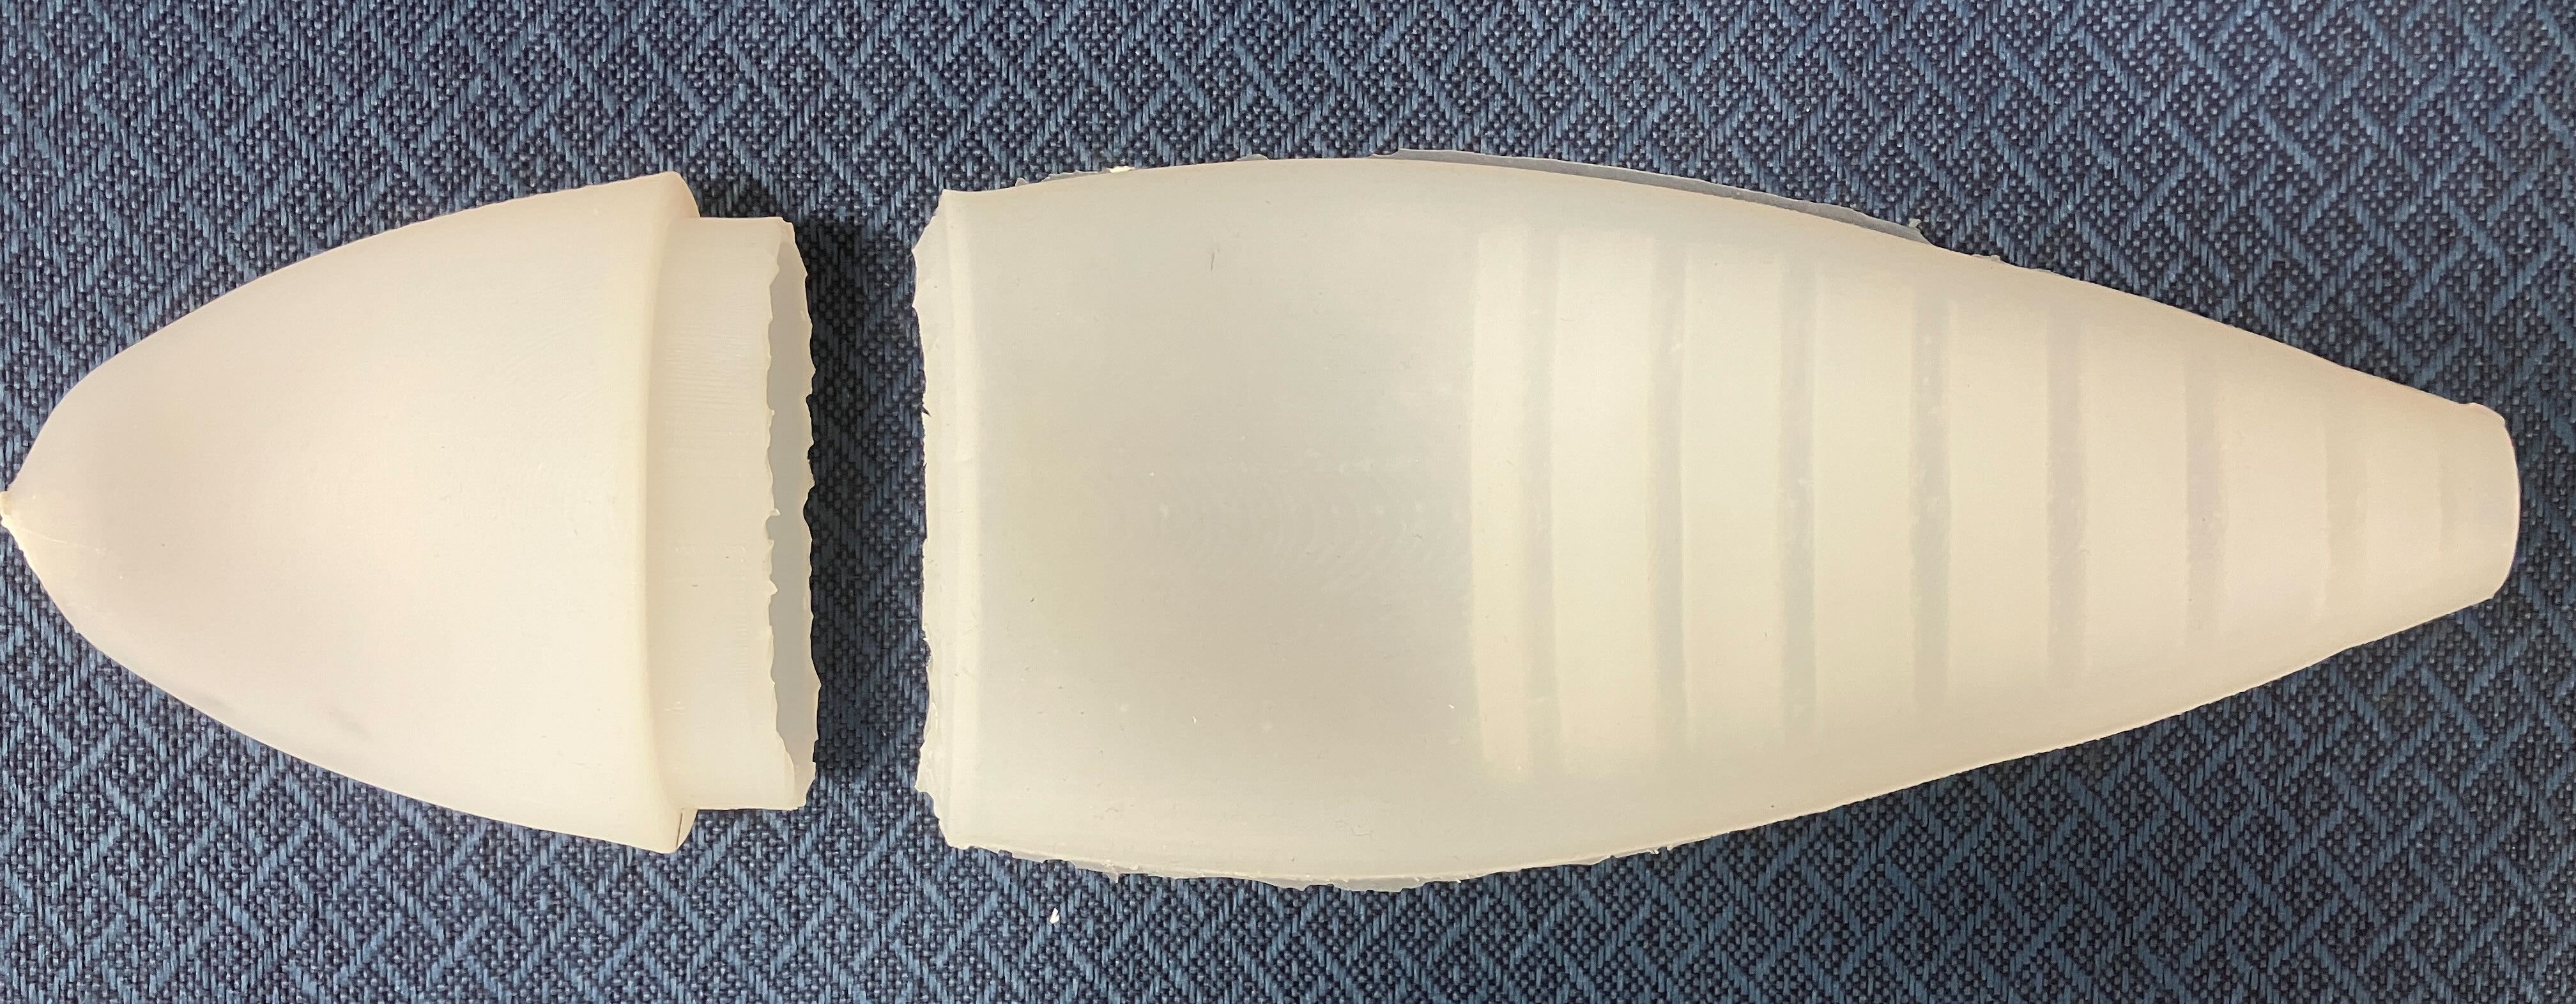
\includegraphics[width=0.6\linewidth]{chapters/picture/gaihi.jpg}
    \caption{作製した外皮}
    \label{fig:gaihi}
\end{figure}